De XOR\index{XOR} geeft alleen als \'e\'en van beide ingangen 1 is een 1 op de uitgang. De XOR functie wordt veel gebruikt in de cryptografie\index{Cryptografie}.

\rowcolors{2}{gray!10}{gray!20}
\begin{tabular}{ |c|c|c| }
\hline
\rowcolor{gray!60}
	Input 1 & Input 2 & Output \\
	\hline
	0 & 0 & 0 \\
	\hline
	0 & 1 & 1 \\
	\hline
	1 & 0 & 1 \\
	\hline
	1 & 1 & 0 \\
	\hline
\end{tabular}

Het symbool voor de XOR is weergegeven in figuur \ref{symbool:xor}

\begin{figure}[h]
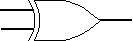
\includegraphics{xor_symbool}
\centering
\caption{Symbool van een XOR}
\label{symbool:xor}
\end{figure}

Er zijn vele manieren om een XOR te bouwen, er is dan ook geen circuit opgenomen. Zie Wikipedia voor mogelijke oplossingen.

In de wiskunde of in programmeertalen kan je de XOR tegenkomen met de volgende symbolen:
\begin{math}
\oplus \; 
\end{math}
